\documentclass[Ex4_Zusammenfassung.tex]{subfiles}

\begin{document}
\section{Tiefinelastische Streuung}
\textbf{von S\o{}ni \& Martina}\\

Bei festen $q^2$ und $\nu$ kann $\tan^2 \frac{\theta}{2}$ auf der X--Achse und $2W_1\lp q^2,\nu\rp \tan^2 \frac{\theta}{2} + W_2\lp q^2,\nu\rp$ auf der Y--Achse aufgetragen werden. Daraus lässt sich folgender Zusammenhang schreiben:
\begin{equation}
	y(x) = 2W_1x+W_2
\end{equation}

Wir wollen aus Messungen die Strukturfunktionen $F$ bestimmen:
\begin{align}
	F_1\lp x,q^2\rp &= Mc^2 W_1\lp q^2,\nu\rp\\
	%%
	F_2\lp x,q^2\rp &= \nu W_2\lp q^2,\nu\rp
\end{align}
Diese sind dimensionslose Strukturfunktionen, wobei $\nu$ den Energieübertrag (da inelastische Streuung; bei elastischer Streuung nur Impulsübertrag) und $x$ die Bjorken'sche Skalenvariable (Inelastizität der Streuung) beschreiben. $x$ ist definiert durch:
\begin{equation}
	x = \frac{-q^2}{2M\nu}
\end{equation}

\subsection*{Wirkungsquerschnitt}
\begin{equation}
	\derive{^2 \sigma}{\lp q^2\rp \md x} = \frac{4\pi \alpha}{q^4} \lp \lp 1-y\rp \frac{F_2}{x} + y^2 F_2\rp
\end{equation}
wobei $y=\frac{\nu}{E}$ den relativen Energieübertrag darstellt.
\pagebreak
\subsection*{Tiefinelastische Streuung}
Nun wollen wir uns mit der Frage beschäftigen, wie die Struktur innerhalb eines Kernes aussieht. Für Energien groß genug dringen die Streuteilchen in den Kern ein. Somit lässt sich die tiefinelastische Streuung als elastische Streuung an \textbf{Partonen} = ''Konstituenten des Nukleus'' beschreiben.
\begin{figure}[H]
	\centering
	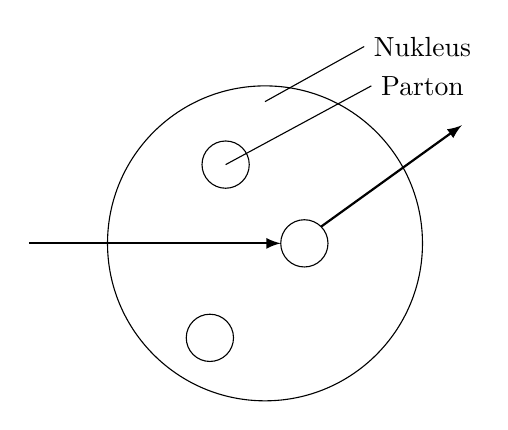
\begin{tikzpicture}
		%defs
		\def\ra{0.3cm}
		%nodes
		\node at (2,2.5) (nuk) {Nukleus};
		\node at (2, 2) (par) {Parton};
		%shapes
		\draw (0,0) circle (2cm);
		\draw (0.5,0) circle (\ra);
		\draw (-0.5,1) circle (\ra);
		\draw (-0.7,-1.2) circle (\ra);
		%lines
		\draw (nuk.west) -- (0,1.8);
		\draw (par.west) -- (-0.5,1);
		\draw [thick, ->, >=latex] (-3,0) -- (0.2,0);
		\draw [thick, ->, >=latex] (0.712,0.212) -- (2.5,1.5);
	\end{tikzpicture}
	\caption{Schema der elastischen Streuung an Partonen}
\end{figure}

\subsection*{Quasielastische Streuung an punktförmigen Teilchen}
Experimentell können wir folgendes ermitteln:
\begin{itemize}
	\item $F_1$ \& $F_2$ hängen nicht von $q^2$ ab
	\item $x$ ist konstant
\end{itemize}

%\begin{figure}
%	\centering
%	\begin{tikzpicture}
%		\begin{feynman}
%		
%		
%		\end{feynman}
%	\end{tikzpicture}
%\end{figure}
\end{document}